\documentclass[conference]{IEEEtran}
\IEEEoverridecommandlockouts
% The preceding line is only needed to identify funding in the first footnote. If that is unneeded, please comment it out.
\usepackage{cite}
\usepackage{amsmath,amssymb,amsfonts}
\usepackage{algorithmic}
\usepackage{graphicx}
\usepackage{textcomp}
\usepackage{xcolor}
\usepackage{multirow}
\usepackage{tabularray}
\usepackage{float}
\usepackage{booktabs}
\usepackage[group-separator={,}]{siunitx}
\def\BibTeX{{\rm B\kern-.05em{\sc i\kern-.025em b}\kern-.08em
    T\kern-.1667em\lower.7ex\hbox{E}\kern-.125emX}}
\begin{document}

\title{Weakly Supervised Object Detection Using Class Activation Map\\
    % {\footnotesize \textsuperscript{*}Note: Sub-titles are not captured in Xplore and
    % should not be used}
}

\author{Anonymous Author Submission}

\maketitle

\begin{abstract}
    Class activation map helps visualize the region of a given object category in an image that an accurate classifier uses for prediction. The original work also extended this method to solve weakly supervised object localization. However, results have shown that class activation map only shows the discriminative part of an object instead of the whole object. Recent proposed solutions help alleviate this problem and allow class activation map to achieve state-of-the-art localizing performance. In this paper, we take advantage of those solutions and propose modifications to use CAM for detecting multiple objects instead.
\end{abstract}

\begin{IEEEkeywords}
    class activation map, weakly supervised object detection
\end{IEEEkeywords}

\section{Introduction}
Class Activation Map (CAM) introduced by Zhou et al. \cite{zhou2015cnnlocalization} to visualize the region of a given object category in an image. This method utilizes the weights from the fully connected layer and the feature maps before the global average pooling layer to generate CAM. CAM allows us to know which region of the image is used by an accurate classifier to make a prediction. Zhou et al. extended their work to solve weakly supervised object localization (WSOL). WSOL aims to find a region of a targeted object in an image using image-level labels as training data. Weakly supervised approaches are great alternatives to fully supervised approaches \cite{Jocher_YOLO_by_Ultralytics_2023} \cite{ren2015faster} as they require less effort and cost to collect, label, and train data.

However, research has shown that CAM only highlights the most discriminative part of an image, thus affecting the localization performance. Kim et al. \cite{kim2022bridging} solved this problem by addressing issues when training a classifier to generate CAM. The proposed method expands the discriminative region to the whole object, thus achieving state-of-the-art localization performance on ImageNet-1k \cite{ILSVRC15} and CUB-200-2011 \cite{WahCUB_200_2011}. Another solution from Yang et al. \cite{yang2019combinational} is to use a function to combine CAM from different categories.

Although the discriminative part has been solved, CAM only focuses on finding the region of a single object. Utilizing Kim et al. \cite{kim2022bridging} work, we propose modifications to use CAM for object detection instead of object localization.

In summary, the contributions of this paper are as follows:
\begin{itemize}
    \item We propose a way to extend \cite{kim2022bridging} for object detection instead of object localization.
    \item We show how using Otsu as a post-processing step can affect the result of the proposed method.
\end{itemize}

\section{Related Works}
\textbf{Weakly Supervised Object Detection (WSOD).} WSOD has gained significant attention as it aims to localize and detect objects using only image-level labels during training, alleviating the need for costly instance-level annotations. Existing WSOD approaches can be broadly categorized into two main paradigms: Multiple Instance Learning (MIL) based and CAM based methods.

\textbf{MIL-based}
MIL-based techniques \cite{DBLP:journals/corr/BilenV15}, \cite{tang2017multiple}, \cite{wang2022d2df2wod}, \cite{huang2022w2nswitching} treat an image as a bag of region proposals or instances, where at least one instance should contain the object of interest. These methods iteratively learn to classify the proposals and refine the object localization.

\textbf{CAM-based}
On the other hand, CAM-based approaches \cite{zhou2015cnnlocalization}, \cite{kim2022bridging}, \cite{yang2019combinational} leverage class activation maps generated from classification networks to localize discriminative object regions. However, vanilla CAM often highlights only the most discriminative parts rather than full object extents. Several works have proposed solutions to this issue, either by introducing auxiliary losses [Kim et al., 2022] to encourage complete object activation or by combining activation maps across categories [Yang et al., 2019].

Our proposed multi-label formulation is motivated by the fact that many object detection datasets contain images with multiple object categories present. By extending CAM to multi-label classification, we aim to improve the localization performance of WSOD methods on such datasets.

\section{Preliminary}
\subsection{Class Activation Map}
CAM is acquired by first training a multi-class classifier with a global average pooling (GAP) layer between the last convolutional layer and the fully connected (FC) layer with softmax as activation function \cite{zhou2015cnnlocalization}. The prediction loss is calculated by cross-entropy (CE) function:

\begin{equation}\label{eq:ce_loss}
    \mathcal{L}_{\text{CE}}=-\sum_{i}^{C}{y_i log(s_i)}
\end{equation}
with $y_i \in \{0, 1\}$ is the ground truth label and $s_i$ is the logit of the $i$-th class.

CAM is then generated by taking the weighted sum of the feature maps from the last convolutional layer with the weights from the FC layer:

\begin{equation}\label{eq:cam}
    \text{CAM}(x)=\mathbf{w}_c^{\boldsymbol{\top}} F(x)
\end{equation}
where $\mathbf{w}_c$ is the weight of the $c$-th class and $F(x) \in \mathbb{R}^{H \times W \times D}$ is the feature map of the last convolutional layer.

However, it is widely observed that CAM only highlights the most discriminative part of an object. This drawback affects the localization performance of CAM thus detection performance also affected.


\subsection{Bridging the Gap between Classification and Localization for Weakly Supervised Object Localization}
Although CAM is generated from an accurate classifier, the classification performance does not translate to localization performance. To address this issue, Kim et al. \cite{kim2022bridging} first interpreted CAM as the degree of aligment between the direction of input features and the direction of class-specific vectors.

Kim et al. interpreted from Eq. \ref{eq:cam} that the value of CAM at each spatial location $u \in \{1, \dots, HW\}$ is the dot product between the feature map at that location and the weight of the class. From that, they decomposed Eq. \ref{eq:cam} further:

\begin{equation} \label{eq:cam at spatial location}
    \begin{split}
        \text{CAM}_u(x) & = \mathbf{w}_c \cdot F_u(x)                                                                                                                \\
                        & = ||\mathbf{w}_c|| ~ || F_u(x) || ~ \underbrace{\frac{\mathbf{w}_c \cdot F_u(x)}{||\mathbf{w}_c|| ~ ||F_u(x)||}}_{S(\mathbf{w}_c, F_u(x))} \\
    \end{split}
\end{equation}
where $S(a, b)$ is the cosine similarity between two vectors $a$ and $b$. From this decomposition, the value at each spatial location $u$ is the product between the norm of a class-specific weight and the norm of the feature map at that location, and the cosine similarity between the two vectors. Eq. \ref{eq:cam at spatial location} can be rewritten as:

\begin{equation} \label{eq:cam with norm and similarity}
    \text{CAM} = ||\mathbf{w}_c|| \cdot \mathcal{F} \odot \mathcal{S}
\end{equation}
with $\mathcal{F} \in \mathbb{R}^{H\times W}$ and $\mathcal{S} \in \mathbb{R}^{H\times W}$ be the norm map and similarity map, respectively, where $\mathcal{F}_u = ||F_u||$ and \\ $\mathcal{S}_u = S(\mathbf{w}_c, F_u(x))$.

Likewise, the classification score calculated from GAP output, $f(x) = GAP(F(x)) \in \mathbb{R}^D$ can be formulated as:
\begin{equation} \label{eq:logit with norm and similarity}
    \begin{split}
        \text{logit}_c(x) & = \mathbf{w}_c \cdot f(x)                             \\
                          & = ||\mathbf{w}_c|| ~ ||f(x)|| ~ S(\mathbf{w}_c, f(x))
    \end{split}
\end{equation}

Because $f(x)$ is fixed for $x$, the scale variation of $||\mathbf{w}_c||$ across each class $c$ is not large so the similarity between $||mathbf{w}_c||$ and $f(x)$ need to be large for $c$ to be predicted. Here, Kim et al. found that the classifier is trained to maximize the similarity between weights of a class and the output of the GAP. This lead to the model only localize discriminative part of the object. To brigde this gap, Kim et al. proposed two method: align feature directions and consistency with attentive dropout. The former method introduce two loss that complement each other: norm loss and similarity loss. The latter method introduce a dropout layer to the model architecture when training.

\begin{figure*}
    \centering
    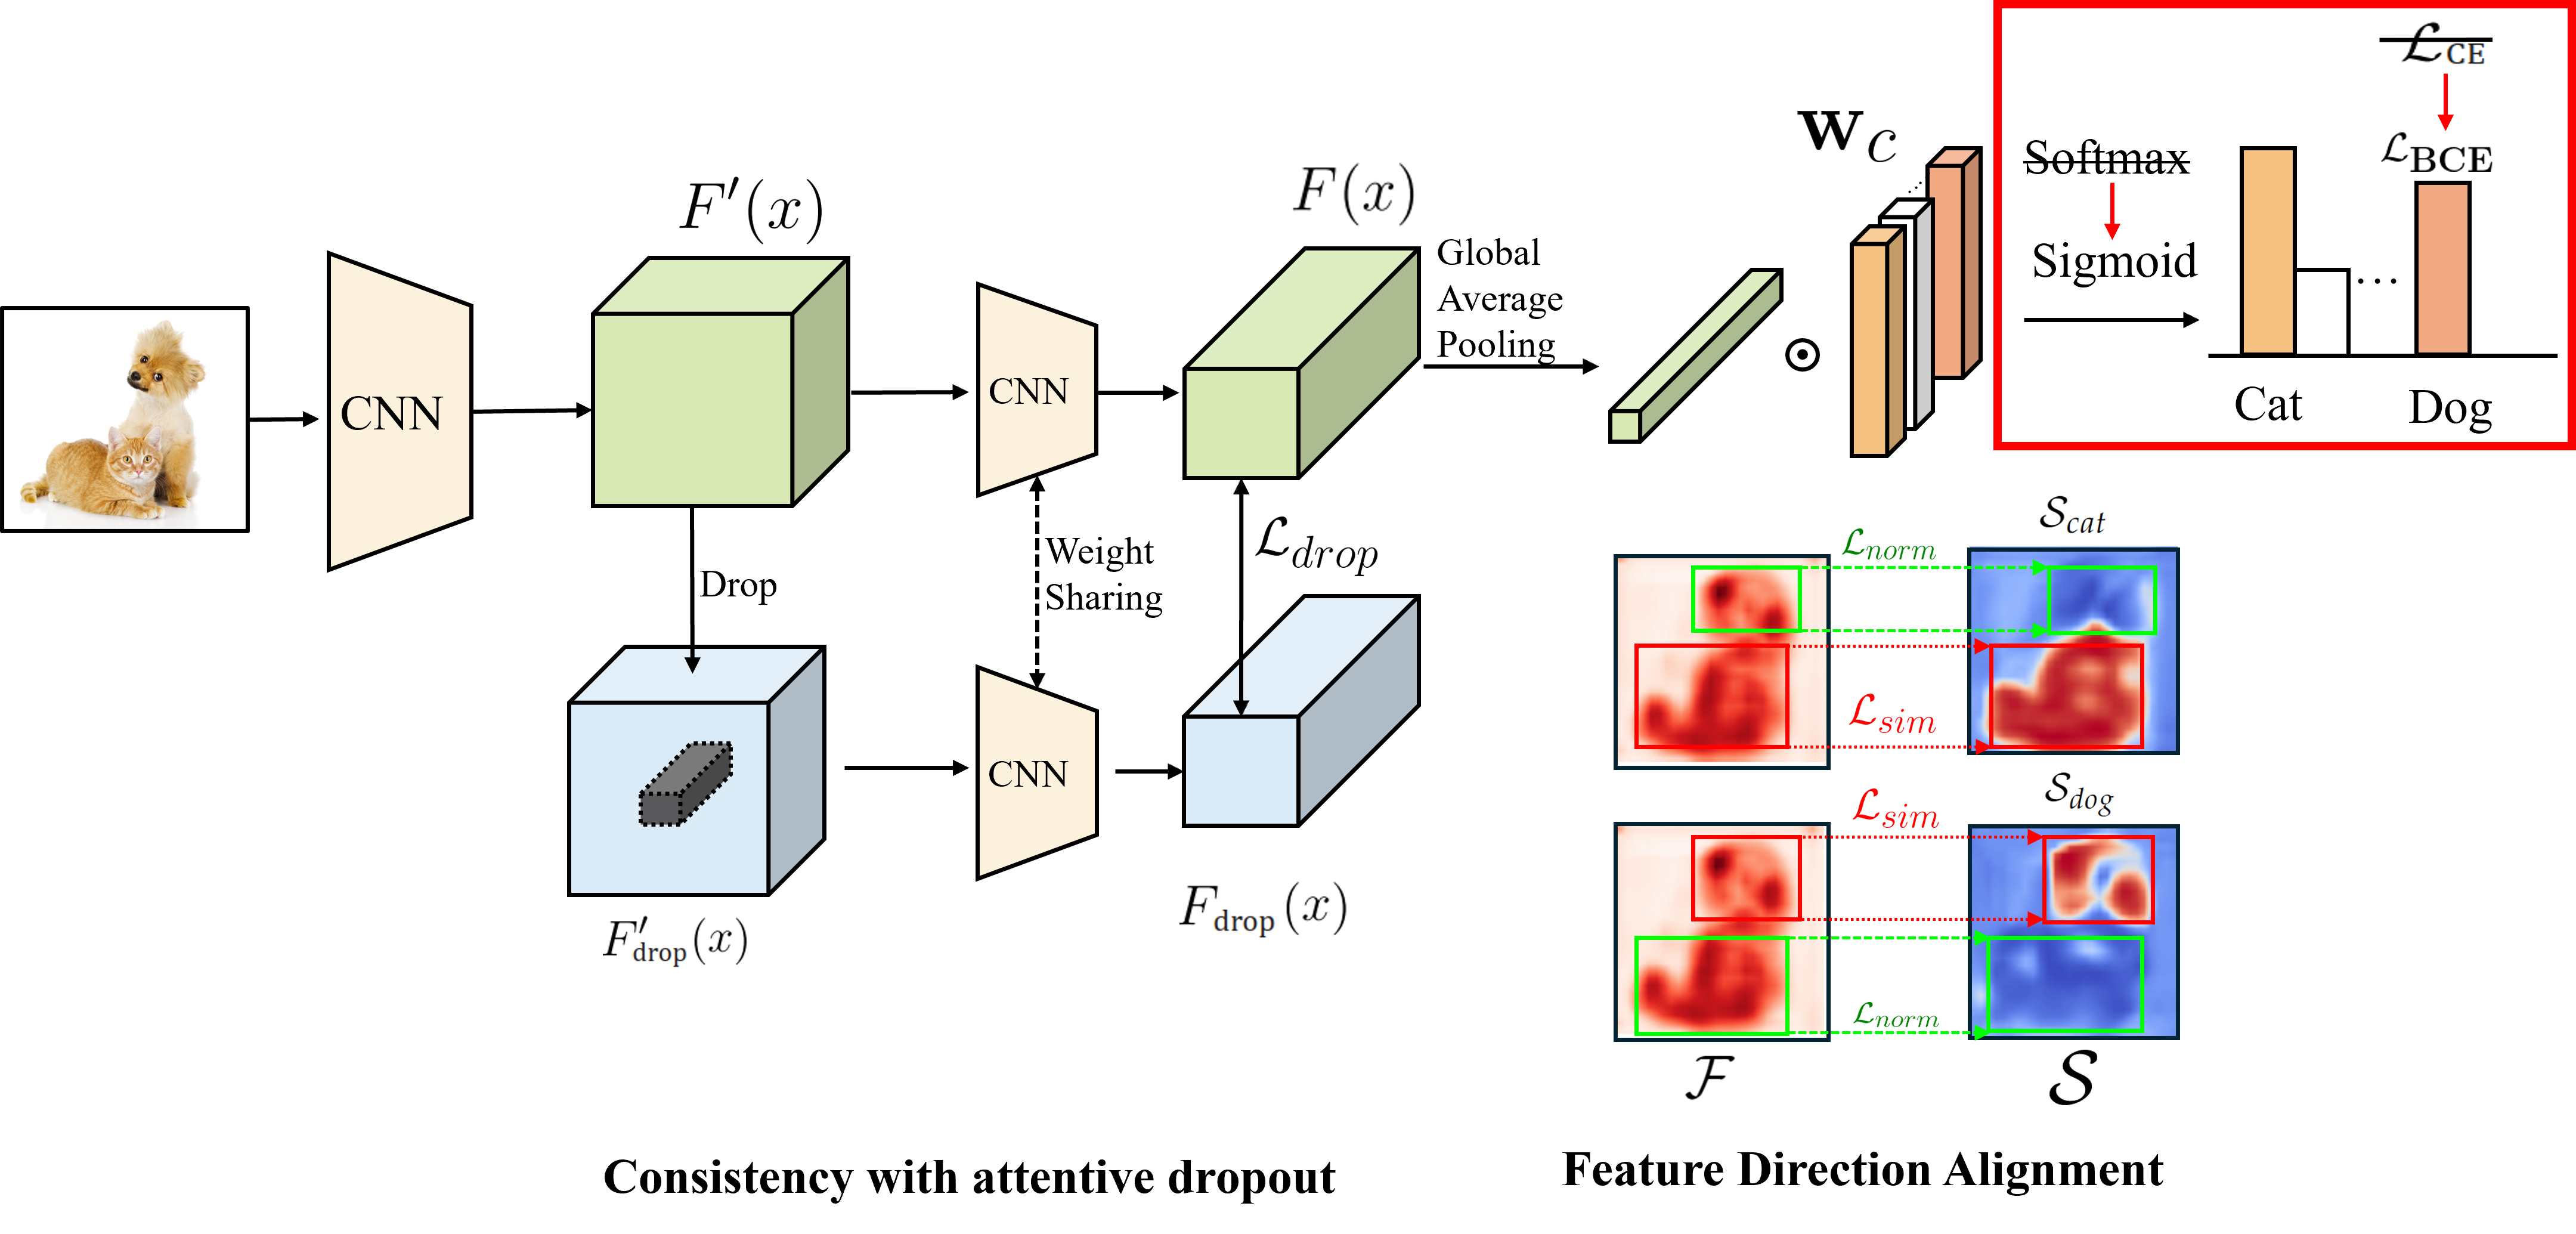
\includegraphics[width=0.95\textwidth]{Figures/architecture.png}
    \caption{The proposed modification to Kim et al. \cite{kim2022bridging} work}
    \label{fig:architecture}
\end{figure*}

\subsubsection{Similarity loss}
Similarity loss aims to increasing the similarity in foreground region and suppress it in background region based on high and low value region on a normalized $\mathcal{F}$. Similarity loss helps expand the activation region to the whole object.

\begin{gather} \label{eq:sim loss}
    \begin{aligned}
         & \mathcal{R}_{\text{fg}}^{\text{norm}} = \{u|\hat{\mathcal{F}_u} > \tau_{\text{fg}}\},                                        & \\
         & \mathcal{R}_{\text{bg}}^{\text{norm}} = \{u|\hat{\mathcal{F}_u} < \tau_{\text{bg}}\},                                        & \\
         & \text{where} ~ \hat{\mathcal{F}} = \frac{\mathcal{F} - \min_i{\mathcal{F}_i}}{\max_i{\mathcal{F}_i} - \min_i{\mathcal{F}_i}} &
    \end{aligned}\\
    \mathcal{L}_{\text{sim}} = -\frac{1}{|\mathcal{R}_{\text{fg}}^{\text{norm}}|} \sum_{u\in\mathcal{R}_{\text{fg}}^{\text{norm}}}{\mathcal{S}_u} + \frac{1}{|\mathcal{R}_{\text{bg}}^{\text{norm}}|} \sum_{u\in\mathcal{R}_{\text{bg}}^{\text{norm}}}{\mathcal{S}_u}
\end{gather}

\subsubsection{Norm loss}
Norm loss aims to active area in object region and suppress in background region in $\hat{\mathcal{F}}$ based on positive and negative region estimated from $S_u$.

\begin{gather} \label{eq:norm loss}
    \begin{aligned}
         & \mathcal{R}_{\text{fg}}^{\text{sim}} = \{u|\mathcal{S}_u>0\}, & \\
         & \mathcal{R}_{\text{bg}}^{\text{sim}} = \{u|\mathcal{S}_u<0\}  &
    \end{aligned} \\
    \mathcal{L}_{\text{norm}} = -\frac{1}{|\mathcal{R}_{\text{fg}}^{\text{sim}}|}\sum_{u\in\mathcal{R}_{\text{fg}}^{\text{sim}}}{\hat{\mathcal{F}_u}} + \frac{1}{|\mathcal{R}_{\text{bg}}^{\text{sim}}|}\sum_{u\in\mathcal{R}_{\text{bg}}^{\text{sim}}}{\hat{\mathcal{F}_u}}
\end{gather}


\subsubsection{Consistency with Attentive Dropout}
Kim et al. \cite{kim2022bridging} introduces a dropout layer between the backbone's layer in the training process. This dropout layer stochastically dropping the activation of an itermediate feature map $\mathcal{F}'$ at the spatial location of whose channel-wised average value is highers than a threshold. Then $\mathcal{F}'$ is passed through the rest of the model's backbone to attain $\mathcal{F}_{drop}$. Finally, $\mathcal{L}_1$ loss is calculated between $\mathcal{F}_{drop}$ and $\mathcal{F}$.

\begin{equation} \label{eq:drop loss}
    \mathcal{L}_{drop} = ||F(x) - F(x)_{drop}||_1
\end{equation}

\subsubsection{Training Scheme}
The final loss function is the combination of CE loss, similarity loss, norm loss, and dropout loss:

\begin{equation} \label{eq:total loss}
    \mathcal{L}_{total} = \mathcal{L}_{\text{CE}} + \lambda_{\text{sim}}\mathcal{L}_{\text{sim}} + \lambda_{\text{norm}}\mathcal{L}_{\text{norm}} + \lambda_{\text{drop}}\mathcal{L}_{\text{drop}}
\end{equation}

The model need to be trained for a few epoch without the feature direction alignment loss in order to stabilize feature map for classification. Then, the feature direction alignment loss is added to the total loss function.

\begin{equation}
    \mathcal{L}_{warm} = \mathcal{L}_{\text{CE}} + \lambda_{\text{drop}}\mathcal{L}_{\text{drop}}
\end{equation}

% \subsection{CCAM}

% Yang et al. \cite{yang2019combinational} proposed a method to combine CAM from different categories.

% Briefly describe the method.

% We propose to use one of the solutions proposed by this method to improve CAM performance.


\section{Proposed Method}
\subsection{From multi-class to multi-label}
In the original work by Zhou et al. \cite{zhou2015cnnlocalization}, CAMs were inferred from a multi-class classifier. This approach, which utilizes a softmax activation function and CE loss, is not well-suited for multi-label data. To address this limitation, we propose a multi-label classification framework for CAM generation. This framework employs a sigmoid activation function $\frac{1}{1 + e^{-x}}$ in the final layer, enabling the model to predict the presence or absence of multiple classes simultaneously. Binary cross-entropy (BCE) loss is then used as the loss function during training to optimize these predictions:

\begin{equation}
    \mathcal{L}_{\text{BCE}} = -\sum_{i}^{C}{y_i \log(\sigma(s_i))}
\end{equation}

We also train both original multi-class architecture \cite{zhou2015cnnlocalization} \cite{kim2022bridging} on multi-label dataset to compare with our proposed modification. To achieve this, with each image containing multiple labels, we add duplicate images for each label. For example, an image with labels \{cat, dog\} will be duplicated into two images: one with label cat and another with label dog. This way, the model can learn to predict each label independently and CE loss can be used as proposed by both original works.

\begin{figure*}
    \centering
    \begin{tblr}{
            width = 0.95\textwidth,
            colspec = {X[-1,m,c] X[c,h] X[c,h] X[c,h] X[c,h] X[c,h]},
            stretch = 0,
        }
        {Global                                                       \\ Thresholding} & 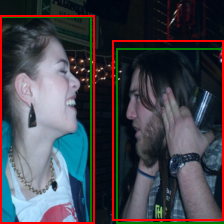
\includegraphics[width=\linewidth]{Figures/475_0_person_threshold.png}      & 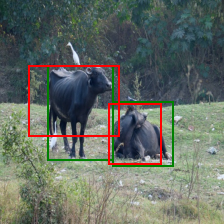
\includegraphics[width=\linewidth]{Figures/499_2_cow_threshold.png}      & 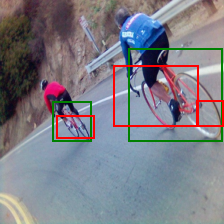
\includegraphics[width=\linewidth]{Figures/259_4_bicycle_threshold.png}   & 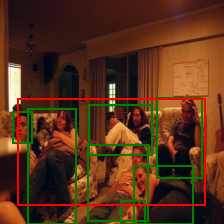
\includegraphics[width=\linewidth]{Figures/3_4_person_threshold.png} & 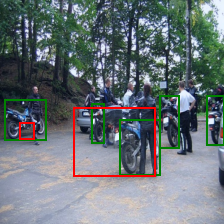
\includegraphics[width=\linewidth]{Figures/208_2_motorbike_threshold.png}\\
        {Otsu                                                         \\ Thresholding} & 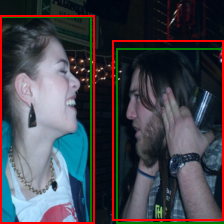
\includegraphics[width=\linewidth]{Figures/475_0_person_otsu_threshold.png} & 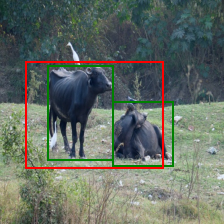
\includegraphics[width=\linewidth]{Figures/499_2_cow_otsu_threshold.png} & 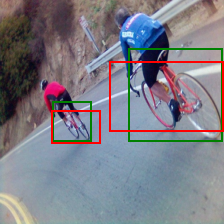
\includegraphics[width=\linewidth]{Figures/259_4_bicycle_otsu.png}        & 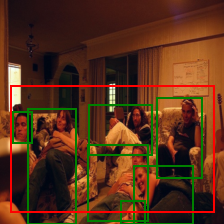
\includegraphics[width=\linewidth]{Figures/3_4_person_otsu_threshold.png} & 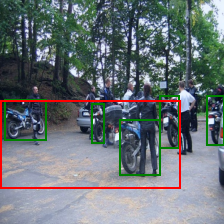
\includegraphics[width=\linewidth]{Figures/208_2_motorbike_otsu_threshold.png}\\
        {CAM                                                          \\ }             & 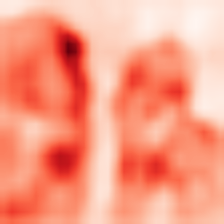
\includegraphics[width=\linewidth]{Figures/475_0_person_cam.png}            & 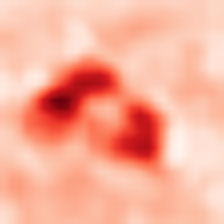
\includegraphics[width=\linewidth]{Figures/499_2_cow_cam.png}            & 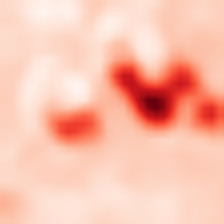
\includegraphics[width=\linewidth]{Figures/259_4_bicycle_cam.png}         & 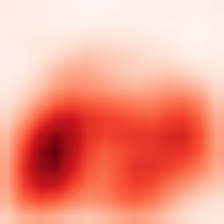
\includegraphics[width=\linewidth]{Figures/3_4_person_cam.png} & 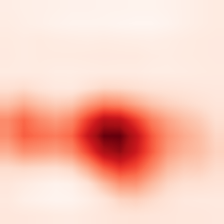
\includegraphics[width=\linewidth]{Figures/208_2_motorbike_cam.png}\\
         & a) person & b) cow & c) bicycle & d) person & e) motorbike \\
    \end{tblr}
    \caption{Comparison between global thresholding, Otsu thresholding. Green boxes denote ground truth, red boxes denote predicted bounding boxes.}
    \label{fig:img result}
\end{figure*}

\subsection{Architecture}
We use most of the architecture from Kim et al. \cite{kim2022bridging} work. Fig. \ref{fig:architecture}. show our proposed modification. We modify the fully connected layer to predict the presence or absence of multiple classes using sigmoid activation function. However, both norm loss and similarity loss are class-specific, so we need to modify the loss function to accommodate multi-label classification. The modification is simply average the loss of each present class:

\begin{gather} \label{eq:modified loss}
    \begin{align}
        \mathcal{L}'_{\text{sim}} = \frac{1}{n}\sum_{i}^{c}y_i (-\frac{1}{|\mathcal{R}_{\text{fg}}^{\text{norm}}|} \sum_{u\in\mathcal{R}_{\text{fg}}^{\text{norm}}}{\mathcal{S}_u} + \frac{1}{|\mathcal{R}_{\text{bg}}^{\text{norm}}|} \sum_{u\in\mathcal{R}_{\text{bg}}^{\text{norm}}}{\mathcal{S}_u}) \\
        \mathcal{L}'_{\text{norm}} = \frac{1}{n}\sum_{i}^{c}y_i (-\frac{1}{|\mathcal{R}_{\text{fg}}^{\text{sim}}|}\sum_{u\in\mathcal{R}_{\text{fg}}^{\text{sim}}}{\hat{\mathcal{F}_u}} + \frac{1}{|\mathcal{R}_{\text{bg}}^{\text{sim}}|}\sum_{u\in\mathcal{R}_{\text{bg}}^{\text{sim}}}{\hat{\mathcal{F}_u}})
    \end{align}
\end{gather}
where $n$ is the number of present classes and $y_i \in \{0, 1\}$ is the groundtruth for each class.

We also modify the total loss function Eq. \ref{eq:total loss} to accommodate multi-label classification by changing CE loss to BCE loss:

\begin{equation}
    \mathcal{L}'_{\text{total}} = \mathcal{L}_{\text{BCE}} + \lambda_{\text{sim}}\mathcal{L}'_{\text{sim}} + \lambda_{\text{norm}}\mathcal{L}'_{\text{norm}} + \lambda_{\text{drop}}\mathcal{L}_{\text{drop}}
\end{equation}


\subsection{Post processing}
\subsubsection{Threshold method}
After accquiring CAM, followed Zhou et al. \cite{zhou2015cnnlocalization}, Kim et al. employed a thresholding technique to segment the CAM, retaining only regions with values exceeding a predefined threshold (e.g., 20\%). Then the bounding box covering the contour of the segmented region is extracted as the object localization. However, this thresholding technique is sensitive to the choice of threshold, every CAM may require a different threshold to achieve optimal segmentation. We propose an alternative post-processing step utilizing Otsu's method \cite{otsu}. This method offers a data-driven approach to threshold selection, potentially leading to more robust CAM segmentation. We apply Gaussian filtering to the CAM to reduce noise before applying Otsu's method. The resulting binary image is then used to extract the bounding box.

To acquire the original threshold method \cite{zhou2015cnnlocalization} result, we run evaluation on multiple threshold $0 \leq \tau < 1$ and report the highest result. As for Otsu's method, the Gaussian filter requires a kernel size $k$. We run evaluation on multiple $k$ and report the highest result.



\subsubsection{Bounding box generation}
Kim et al. \cite{kim2022bridging} utilize all contours for bounding box generation. However, in certain scenarios, imperfect CAM segmentation can introduce background regions within the object area. This results in two bounding boxes: one encompassing the outer region's contour and another for the inner region. We propose leveraging the bounding box generated from the external contour to represent the object of interest.

\subsubsection{Confidence score}
Another issue is that confidence score, typically output by object detection models, for each bounding box is not calculated. This lead to difficulty in evaluating the model's performance with COCO mAP \cite{lin2015microsoft}. For the time being, we use class probabilities output by model FC layer as confidence score.



\begin{table}[t]
    \centering
    \caption{classification result on VOC 2007}
    \label{tab:classification_map_voc_2007}
    \begin{tabular}{|c|l|c|c|}
        \hline
        Backbone                     & Method                                              & Val                             & Test                            \\
        \hline
        \multirow[c]{4}{*}{ResNet50} & CAM\cite{zhou2015cnnlocalization}                   & 80.09\%                         & 81.12\%                         \\
                                     & Kim et al. \cite{kim2022bridging}                   & 77.86\%                         & 77.71\%                         \\
                                     & CAM\cite{zhou2015cnnlocalization} + BCE loss (ours) & \color{red} \bfseries{84.69\%}  & \color{red} \bfseries{84.33\%}  \\
                                     & Kim et al. \cite{kim2022bridging} + BCE loss (ours) & 81.92\%                         & 81.59\%                         \\
        \hline
        \multirow[c]{4}{*}{VGG16}    & CAM\cite{zhou2015cnnlocalization}                   & \color{blue} \bfseries{77.07\%} & \color{blue} \bfseries{78.00\%} \\
                                     & Kim et al. \cite{kim2022bridging}                   & 75.18\%                         & 76.14\%                         \\
                                     & CAM\cite{zhou2015cnnlocalization} + BCE loss (ours) & 74.95\%                         & 75.80\%                         \\
                                     & Kim et al. \cite{kim2022bridging} + BCE loss (ours) & 75.88\%                         & 75.89\%                         \\
        \hline
    \end{tabular}
\end{table}

\section{Experiments}
\subsection{Experimental Setup}
\textbf{Dataset.} We perform our modifications on two popular multi-label classification datasets: PASCAL VOC 2007 \cite{pascal-voc-2007} and 2012 \cite{pascal-voc-2012}. There are \num{9963} images in VOC 2007 and \num{11530} images in VOC 2012 which are splitted 50:50 to train/val and test.  Each image contains one or multiple labels from 20 categories.

\textbf{Metric.} We use mAP to evaluate classification performance. mAP is the average of each categories' area under precision and recall curve. For detection, we evaluate using a widely known COCO metric: mAP \cite{lin2015microsoft}.

\textbf{Implementation Details.} We adopt ResNet50 \cite{7780459} and VGG16 \cite{simonyan2015deep} as our backbone. We follow network architecture, hyperparameters setting of the previous work \cite{kim2022bridging}. We resize all images to $224\times224$ before passing to the model. Both backbones are initialized with ImageNet-1k \cite{ILSVRC15} pretrained weights. Each model is trained for 50 epochs with SGD optimizer, learning rate of $0.0001$, weight decay of $0.001$, momentum of $0.9$, and batch size of 16. The implementation is run on Google Colab with Tesla T4 GPU, 16GB of RAM.


\begin{table}[t]
    \centering
    \caption{classification result on voc 2012}
    \label{tab:classification_map_voc_2012}
    \begin{tabular}{|c|l|c|}
        \hline
        Backbone                     & Method                                              & Val                             \\
        \hline
        \multirow[c]{4}{*}{ResNet50} & CAM\cite{zhou2015cnnlocalization}                   & \color{red} \bfseries{80.18\%}  \\
                                     & Kim et al. \cite{kim2022bridging}                   & 78.50\%                         \\
                                     & CAM\cite{zhou2015cnnlocalization} + BCE loss (ours) & 71.84\%                         \\
                                     & Kim et al. \cite{kim2022bridging} + BCE loss (ours) & 71.53\%                         \\
        \hline
        \multirow[c]{4}{*}{VGG16}    & CAM\cite{zhou2015cnnlocalization}                   & \color{blue} \bfseries{77.78\%} \\
                                     & Kim et al. \cite{kim2022bridging}                   & 75.66\%                         \\
                                     & CAM\cite{zhou2015cnnlocalization} + BCE loss (ours) & 76.55\%                         \\
                                     & Kim et al. \cite{kim2022bridging} + BCE loss (ours) & 58.83\%                         \\
        \hline
    \end{tabular}
\end{table}

\begin{table}[t]
    \centering
    \caption{highest mAP on multiple cam theshold on voc 2007}
    \label{tab:brute_force_cam_threshold_map_voc_2007}
    \begin{tabular}{|c|l|c|c|}
        \hline
        Backbone                     & Method                                              & Val                             & Test                            \\
        \hline
        \multirow[c]{4}{*}{ResNet50} & CAM\cite{zhou2015cnnlocalization}                   & 6.83\%                          & 7.04\%                          \\
                                     & Kim et al. \cite{kim2022bridging}                   & 6.06\%                          & 6.47\%                          \\
                                     & CAM\cite{zhou2015cnnlocalization} + BCE loss (ours) & 7.66\%                          & 7.93\%                          \\
                                     & Kim et al. \cite{kim2022bridging} + BCE loss (ours) & \color{red} \bfseries{8.14\%}   & \color{red} \bfseries{8.40\%}   \\
        \hline
        \multirow[c]{4}{*}{VGG16}    & CAM\cite{zhou2015cnnlocalization}                   & 11.54\%                         & 11.84\%                         \\
                                     & Kim et al. \cite{kim2022bridging}                   & 9.97\%                          & 10.31\%                         \\
                                     & CAM\cite{zhou2015cnnlocalization} + BCE loss (ours) & 10.41\%                         & 11.56\%                         \\
                                     & Kim et al. \cite{kim2022bridging} + BCE loss (ours) & \color{blue} \bfseries{11.61\%} & \color{blue} \bfseries{12.27\%} \\
        \hline
    \end{tabular}
\end{table}



\subsection{Results}

On VOC 2007 (Tab. \ref{tab:classification_map_voc_2007}), the proposed multi-label modifications classifies better than both multi-class model from the original works \cite{zhou2015cnnlocalization} \cite{kim2022bridging} with ResNet50 backbones. However, the performance is lower than the original multi-class model with VGG16 backbone as both multi-class models only predict a single class per image leading to higher precision, thus higher mAP. For object detection (Tab. \ref{tab:brute_force_cam_threshold_map_voc_2007}), the proposed multi-label modifications show modest improvements over the original methods, but the overall mAP values remain quite low across all methods.



Meanwhile, on the VOC 2012 dataset, the results are even less promising. For classification (Tab. \ref{tab:classification_map_voc_2012}), the original methods again outperform the proposed modifications, sometimes by a large margin (e.g. VGG16 backbone with Kim et al. method \cite{kim2022bridging}). For object detection on VOC 2012 (Tab. \ref{tab:brute_force_cam_threshold_map_voc_2012}), while the proposed ResNet50 modification with Kim et al. method \cite{kim2022bridging} achieved the mAP of 8.33\%, it is still very low.


\begin{table}[t]
    \centering
    \caption{highest mAP on multiple cam theshold on voc 2012}
    \label{tab:brute_force_cam_threshold_map_voc_2012}
    \begin{tabular}{|c|l|c|}
        \hline
        Backbone                     & Method                                              & Val                             \\
        \hline
        \multirow[c]{4}{*}{ResNet50} & CAM\cite{zhou2015cnnlocalization}                   & \color{red} \bfseries{8.50\%}   \\
                                     & Kim et al. \cite{kim2022bridging}                   & 7.90\%                          \\
                                     & CAM\cite{zhou2015cnnlocalization} + BCE loss (ours) & 7.12\%                          \\
                                     & Kim et al. \cite{kim2022bridging} + BCE loss (ours) & 8.33\%                          \\
        \hline
        \multirow[c]{4}{*}{VGG16}    & CAM\cite{zhou2015cnnlocalization}                   & \color{blue} \bfseries{14.53\%} \\
                                     & Kim et al. \cite{kim2022bridging}                   & 12.80\%                         \\
                                     & CAM\cite{zhou2015cnnlocalization} + BCE loss (ours) & 12.31\%                         \\
                                     & Kim et al. \cite{kim2022bridging} + BCE loss (ours) & 7.67\%                          \\
        \hline
    \end{tabular}
\end{table}

Tab. \ref{tab:different_gaussian_ksize_map_voc_2007_val}, \ref{tab:different_gaussian_ksize_map_voc_2007_test}, \ref{tab:different_gaussian_ksize_map_voc_2012_val} compare the performance of global thresholding and Otsu thresholding on VOC 2007 and 2012. Our proposed modifications tend to benefit from using Otsu thresholding instead of global thresholding, especially with the ResNet50 backbone. The improvements are modest but consistent across validation and test sets of both datasets. However, the original single-label methods generally suffer a drop in performance when applying Otsu thresholding.

\begin{table}[t]
    \centering
    \caption{Comparison between global thresholding and Otsu thresholding on VOC 2007 (val)}
    \label{tab:different_gaussian_ksize_map_voc_2007_val}
    \resizebox{\linewidth}{!}{
        \begin{tabular}{|c|l|c|c|c|c|}
            \hline
            Backbone                     & Method                                              & 1                    & 7                    & 21                   & 51                   \\
            \hline
            \multirow[c]{4}{*}{ResNet50} & CAM\cite{zhou2015cnnlocalization}                   & \color{red} -5.03\%  & \color{red} -5.03\%  & \color{red} -4.86\%  & \color{red} -3.98\%  \\
                                         & Bridging\cite{kim2022bridging}                      & \color{red} -4.60\%  & \color{red} -4.58\%  & \color{red} -4.44\%  & \color{red} -3.85\%  \\
                                         & CAM\cite{zhou2015cnnlocalization} + BCE loss (ours) & \color{red} -1.54\%  & \color{red} -1.46\%  & \color{red} -1.13\%  & \color{blue} +0.51\% \\
                                         & Bridging\cite{kim2022bridging} + BCE loss (ours)    & \color{red} -1.24\%  & \color{red} -1.21\%  & \color{red} -0.68\%  & \color{blue} +1.02\% \\
            \hline
            \multirow[c]{4}{*}{VGG16}    & CAM\cite{zhou2015cnnlocalization}                   & \color{red} -1.29\%  & \color{red} -1.22\%  & \color{red} -1.17\%  & \color{red} -1.13\%  \\
                                         & Bridging\cite{kim2022bridging}                      & \color{red} -1.32\%  & \color{red} -1.34\%  & \color{red} -1.25\%  & \color{red} -1.12\%  \\
                                         & CAM\cite{zhou2015cnnlocalization} + BCE loss (ours) & \color{blue} +0.14\% & \color{blue} +0.19\% & \color{blue} +0.32\% & \color{blue} +0.63\% \\
                                         & Bridging\cite{kim2022bridging} + BCE loss (ours)    & \color{red} -0.91\%  & \color{red} -0.83\%  & \color{red} -0.68\%  & \color{red} -0.65\%  \\
            \hline
        \end{tabular}
    }
\end{table}

\begin{table}[t]
    \centering
    \caption{Comparison between global thresholding and Otsu thresholding on VOC 2007 (test)}
    \label{tab:different_gaussian_ksize_map_voc_2007_test}
    \resizebox{\linewidth}{!}{
        \begin{tabular}{|c|l|c|c|c|c|}
            \hline
            Backbone                     & Method                                              & 1                   & 7                   & 21                  & 51                   \\
            \hline
            \multirow[c]{4}{*}{ResNet50} & CAM\cite{zhou2015cnnlocalization}                   & \color{red} -5.10\% & \color{red} -5.11\% & \color{red} -4.88\% & \color{red} -3.91\%  \\
                                         & Bridging\cite{kim2022bridging}                      & \color{red} -5.07\% & \color{red} -5.05\% & \color{red} -4.97\% & \color{red} -4.43\%  \\
                                         & CAM\cite{zhou2015cnnlocalization} + BCE loss (ours) & \color{red} -1.52\% & \color{red} -1.38\% & \color{red} -0.96\% & \color{blue} +0.47\% \\
                                         & Bridging\cite{kim2022bridging} + BCE loss (ours)    & \color{red} -0.98\% & \color{red} -0.89\% & \color{red} -0.32\% & \color{blue} +1.49\% \\
            \hline
            \multirow[c]{4}{*}{VGG16}    & CAM\cite{zhou2015cnnlocalization}                   & \color{red} -1.51\% & \color{red} -1.38\% & \color{red} -1.32\% & \color{red} -1.02\%  \\
                                         & Bridging\cite{kim2022bridging}                      & \color{red} -1.58\% & \color{red} -1.57\% & \color{red} -1.53\% & \color{red} -1.37\%  \\
                                         & CAM\cite{zhou2015cnnlocalization} + BCE loss (ours) & \color{red} -0.41\% & \color{red} -0.32\% & \color{red} -0.16\% & \color{blue} +0.25\% \\
                                         & Bridging\cite{kim2022bridging} + BCE loss (ours)    & \color{red} -0.48\% & \color{red} -0.38\% & \color{red} -0.35\% & \color{red} -0.09\%  \\
            \hline
        \end{tabular}
    }
\end{table}

\begin{table}[t]
    \centering
    \caption{ Comparison between global thresholding and Otsu thresholding on VOC 2012 (val) }
    \label{tab:different_gaussian_ksize_map_voc_2012_val}
    \resizebox{\linewidth}{!}{
        \begin{tabular}{|c|l|c|c|c|c|}
            \hline
            Backbone                     & Method                                              & 1                    & 7                    & 21                   & 51                   \\
            \hline
            \multirow[c]{4}{*}{ResNet50} & CAM\cite{zhou2015cnnlocalization}                   & \color{red} -5.37\%  & \color{red} -5.30\%  & \color{red} -5.00\%  & \color{red} -3.59\%  \\
                                         & Bridging\cite{kim2022bridging}                      & \color{red} -1.70\%  & \color{red} -1.61\%  & \color{red} -1.39\%  & \color{red} -0.62\%  \\
                                         & CAM\cite{zhou2015cnnlocalization} + BCE loss (ours) & \color{blue} +0.06\% & \color{blue} +0.09\% & \color{blue} +0.21\% & \color{blue} +0.45\% \\
                                         & Bridging\cite{kim2022bridging} + BCE loss (ours)    & \color{blue} +0.10\% & \color{blue} +0.20\% & \color{blue} +0.28\% & \color{blue} +0.40\% \\
            \hline
            \multirow[c]{4}{*}{VGG16}    & CAM\cite{zhou2015cnnlocalization}                   & \color{red} -1.25\%  & \color{red} -1.18\%  & \color{red} -1.02\%  & \color{red} -0.81\%  \\
                                         & Bridging\cite{kim2022bridging}                      & \color{red} -1.74\%  & \color{red} -1.71\%  & \color{red} -1.66\%  & \color{red} -1.55\%  \\
                                         & CAM\cite{zhou2015cnnlocalization} + BCE loss (ours) & \color{red} -0.18\%  & \color{red} -0.07\%  & \color{blue} +0.11\% & \color{blue} +0.50\% \\
                                         & Bridging\cite{kim2022bridging} + BCE loss (ours)    & \color{red} -0.61\%  & \color{red} -0.56\%  & \color{red} -0.54\%  & \color{red} -0.40\%  \\
            \hline
        \end{tabular}
    }
\end{table}

In Fig. \ref{fig:img result}, we show the result of our proposed modifications. Examples a, b, and c show that both thresholding methods can detect objects reasonably well. Fig. \ref{fig:img result} also shows that each thresholding method contributes to better localizing performance by separating regions of different objects (example b) or merging regions of the same object (example c). However, the result is not as good for objects that are close together (example d) or occluded (example e). In example d, CAM only highlights the region containing a group of people, not each person. This leads to the bounding box encompassing all people in the image. In example e, the proposed modifications predict bounding boxes that do not tightly surround small and occluded motorbikes.


\section{Limitation}
Our research has produced unsatisfied results in some instances: objects in the same class close together, small objects and occlusion. Our experiments have not been successful on images with adjacent objects because the result obtained after binarizing the CAM will produce a region encompassing all objects. This is a drawback of binarizing the CAM and identifying contours for small objects or obscured objects. We haven't looked into these situations or offered any solutions because of time constraints. These drawbacks lead us to conclude that contour detection and binarization of the CAM are insufficiently efficient methods for identifying objects in a picture.

\section{Conclusions}
In this paper, we proposed modifications to the CAM-based method by Kim et al. \cite{kim2022bridging} to enable weakly supervised object detection for multiple objects in an image. Our key contributions were: 1) Extending the CAM framework to multi-label classification by using a sigmoid activation and binary cross-entropy loss, and 2) Experimenting with Otsu's adaptive thresholding method \cite{otsu} as an alternative post-processing step to the fixed global thresholding used in previous works.

Our experiments on the PASCAL VOC 2007 and 2012 datasets demonstrated that the proposed multi-label modifications generally improved object detection performance over the original single-label CAM and Kim et al. methods, especially when using the ResNet50 backbone. However, the overall mAP values remained relatively low across all methods evaluated. We also found that our multi-label variants tended to benefit from using Otsu thresholding, achieving modest but consistent improvements compared to global thresholding.

In the future, we plan to explore more advanced post-processing techniques to improve the accuracy of object localization. We also aim to investigate the use of more sophisticated network architectures and loss functions to further enhance the performance of weakly supervised object detection models.

% \section*{References}

\bibliographystyle{IEEEtran}
\bibliography{IEEEabrv,bibi}

\end{document}
